\documentclass{article}
\usepackage{amsthm}
\usepackage[utf8x]{inputenc}
\usepackage[usenames,dvipsnames]{color}
\author{Simone Gasperoni}
\theoremstyle{plain}
\newtheorem{thm}{Teorema}[] 
\theoremstyle{definition}
\newtheorem{defn}[]{Definizione} % definition numbers are dependent on theorem numbers
\newtheorem{exmp}[thm]{Example} % same for example numbers
\usepackage{dirtytalk}
\usepackage{graphicx}
\usepackage{listings}
\usepackage{color}
\usepackage{hyperref}
\definecolor{dkgreen}{rgb}{0,0.6,0}
\definecolor{gray}{rgb}{0.5,0.5,0.5}
\definecolor{mauve}{rgb}{0.58,0,0.82}

\lstset{frame=tb,
	language=python,
	aboveskip=3mm,
	belowskip=3mm,
	showstringspaces=false,
	columns=flexible,
	basicstyle={\small\ttfamily},
	numbers=none,
	numberstyle=\tiny\color{gray},
	keywordstyle=\color{blue},
	commentstyle=\color{dkgreen},
	stringstyle=\color{mauve},
	breaklines=true,
	breakatwhitespace=true,
	tabsize=3
}

\author{Simone Gasperoni}
\title{Catalogazione DCAT di open data amministrativi e governativi con tecniche di text mining}

\begin{document}

\begin{titlepage}
\begin{center}

\textsc{Laurea magistrale in Ingegneria informatica (D.M. 270)}\\[0.5cm]
\textsc{Università degli studi di Roma Tre}\\[0.5cm]

\hrulefill

{ \huge \bfseries Catalogazione DCAT di open data amministrativi e governativi con tecniche di text mining \\[0.4cm] }
\textsc{\Large Simone Gasperoni}\\[0.5cm]
\vfill
\LaTeX


Roma, Italia
\end{center}
\end{titlepage}


\tableofcontents

\newpage
\section{Introduzione}
\textbf{\textit{I dati sono aperti se chiunque è libero di accederli, usarli, modificarli, e condividerli.}}
\footnotemark
\footnotetext{http://opendefinition.org/od/2.1/en}

\subsection{La filosofia open-data}

Gli aspetti più importanti della filosofia open-data sono:
\begin{itemize}
\item Disponibilità e accesso.
\item Riutilizzo e ridistribuzione: i dati devono essere forniti a condizioni tali da permetterne il riutilizzo e la ridistribuzione. Ciò comprende la possibilità di combinarli con altre basi di dati.
\item Partecipazione universale: tutti devono essere in grado di usare, riutilizzare e ridistribuire i dati.
\end{itemize}

Il movimento open-data si diffuse per la prima volta a seguito della promulgazione della Direttiva sull'Open government del 2009 negli Stati Uniti d'America:
\textit{Fin dove possibile e sottostando alle sole restrizioni valide, le agenzie devono pubblicare le informazioni on line utilizzando un formato aperto (open) che possa cioè essere recuperato, soggetto ad azioni di download, indicizzato e ricercato attraverso le applicazioni di ricerca web più comunemente utilizzate. Per formato open si intende un formato indipendente rispetto alla piattaforma, leggibile dall'elaboratore e reso disponibile al pubblico senza che sia impedito il riuso dell'informazione veicolata.}
\\
In questo contesto è nato il portale Data.gov, creato con l'obiettivo di raccogliere in un unico portale tutte le informazioni rese disponibili dagli enti statunitensi in formato aperto. In Italia il portale che raccoglie i dati aperti della pubblica amministrazione è Dati.gov.it
 
\subsection{Interoperabilità}
Tra le ragioni più importanti della filosofia open data abbiamo l'interoperabilità, vale a dire, la capacità di diversi sistemi e organizzazioni di lavorare insieme. Nel caso specifico degli open data - ovviamente - ci riferiamo alla capacità di combinare una grande quantità di dati da diverse fonti. L'interoperabilità è importante perché permette a componenti diverse di lavorare insieme. L'abilità di rendere ciascun dato un componente e di combinare insieme vari componenti è essenziale per la costruzione di sistemi sofisticati. In assenza di interoperabilità ciò diventa quasi impossibile - come nel mito della Torre di Babele, in cui l'impossibilità di comunicare (e quindi di Inter-operare) dà luogo a un fallimento sistemico della costruzione della torre. Una chiara definizione di \say{apertura} assicura che sia possibile combinare dataset aperti provenienti da fonti diverse in modo adeguato, evitando così la \say{Torre di Babele}.
\\
Il punto cruciale di un bacino di dati (o linee di codice) accessibili e utilizzabili in modo condiviso è il fatto che potenzialmente possono essere liberamente \say{mescolati} con dati provenienti da fonti anch'esse aperte. L'interoperabilità è la chiave per realizzare il principale vantaggio pratico dell'apertura: aumenta in modo esponenziale la possibilità di combinare diverse basi di dati, e quindi sviluppare nuovi e migliori prodotti e servizi.
\footnotemark
\footnotetext{http://opendatahandbook.org/guide/it/what-is-open-data}

\subsection{EuroVoc e JRC-Acquis 3.0}
EuroVoc è un thesaurus multilingue e pluridisciplinare che comprende la terminologia dei settori d'attività dell'Unione europea. Contiene termini in 23 lingue dell'UE. EuroVoc è in linea con le raccomandazioni del W3C e con gli ultimi sviluppi negli standard di classificazione. Il thesaurus EuroVoc viene utilizzato dalle istituzioni dell'Unione europea, dall'Ufficio delle pubblicazioni dell'UE, da parlamenti nazionali e regionali in Europa, come pure da amministrazioni nazionali e utenti privati di tutto il mondo.
\footnotemark
\footnotetext{http://eurovoc.europa.eu}
I descrittori del thesaurus multilingua EuroVoc sono usati da molti parlamentari europei e centri di documentazione per indicizzare manualmente le loro collezioni di documenti, i descrittori assegnati ai documenti sono utilizzati per cercare ed individuare documenti in una gerarchia semantica divisa in 21 domini, 127 sottodomini (microthesauri) e N descrittori.

\subsection{DCAT, DCAT-AP e DCAT-AP-it}
Il DCAT Application Profile (DCAT-AP) fornisce una specifica comune per la descrizione di dati della pubblica amministrazione in Europa, questa specifica è basata sullo standard DCAT: Data Catalog Vocabulary. \footnotemark
\footnotetext{https://www.w3.org/TR/vocab-dcat} 
\\
DCAT è un vocabolario RDF progettato per facilitare l'interoperabilità tra cataloghi di dati pubblicati sul web. DCAT incentiva la pubblicazione decentrata di cataloghi e facilita la ricerca federata di dati tra i siti. Usando lo standard DCAT chi pubblica insiemi di dati incrementa la propria visibilità e favorisce le applicazioni che lavorano su dati e metadati in cataloghi multipli (applicazioni cross-portali).
\\
DCAT-AP-it è la versione italiana di DCAT-AP, il profilo nazionale dei metadati utili per descrivere i dati delle pubbliche amministrazioni, conforme alla specifica di DCAT-AP serve a favorire l'interoperabilità semantica di dati e servizi. DCAT-AP-it è un modello dati pensato per rendere omogenei in tutta la pubblica amministrazione italiana i processi di accesso e scambio delle informazioni tra le istituzioni stesse e tra le istituzioni e i cittadini e le imprese, in coerenza con il relativo framework europeo. L'utilizzo di un modello dati valorizza il patrimonio informativo pubblico nazionale in linea con la Direttiva relativa al riutilizzo dell'informazione del settore pubblico.
\begin{figure}[htbp]
\begin{center}
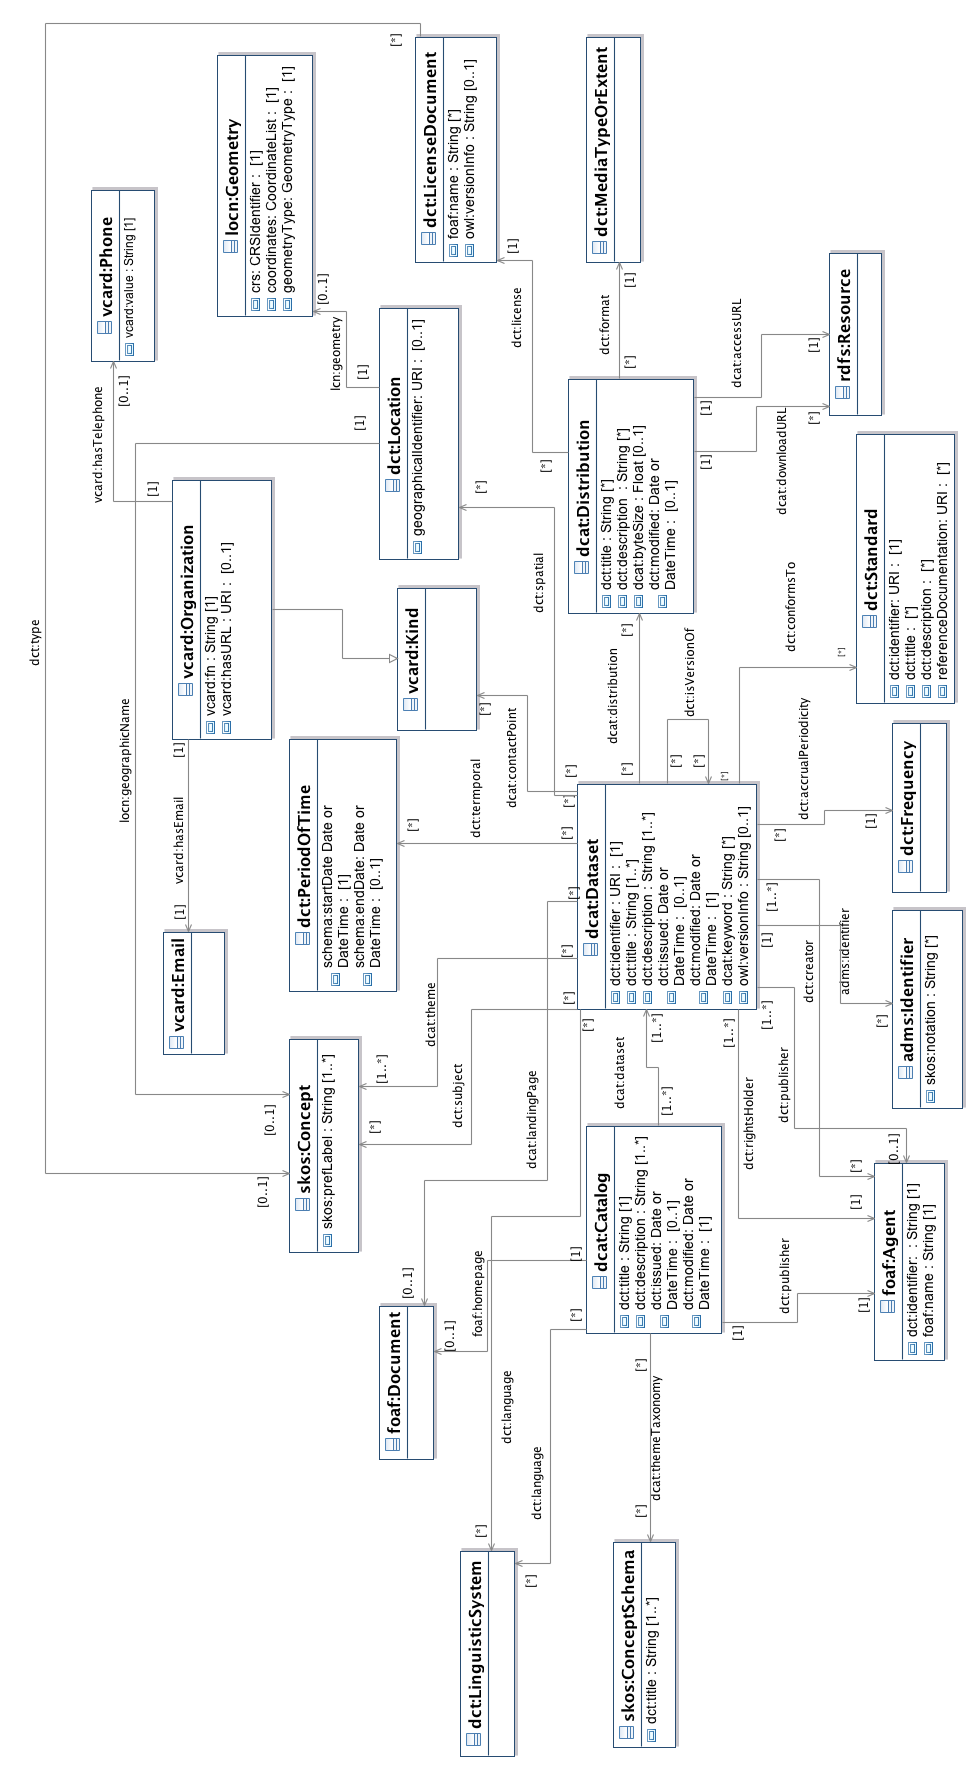
\includegraphics[scale=0.45]{img/DCAT-AP_IT_UML.png}
\caption{Modello dati DCAT-AP-it}
\end{center}
\end{figure}

\newpage
\section{Elaborazione dei corpus}
Una fase preliminare in qualsiasi ambito di classificazione è l'elaborazione dei dati, la loro formattazione, per renderli fruibili da parte di sistema di classificazione.
\\Nel contesto di un sistema di text categorization vogliamo ottenere un sistema che utilizzi feature ben rappresentative del contenuto semantico dei documenti dai quali sono estratte.
\\
Le strade che si possono percorrere sono principalmente due:

\begin{description}
\item [Lemmatizzazione:] \say{quel complesso di operazioni che conducono a riunire tutte le forme sotto il rispettivo lemma}, intendendo per lemma \say{ciascuna parola-titolo o parola-chiave di un dizionario} e per forma ogni possibile diversa realizzazione grafica di un lemma.\footnotemark
\footnotetext{R. Busa, Fondamenti di informatica linguistica. Istituto Geografico De Agostini, 1987}
\\
Esistono delle convenzioni di lemmatizzazione proprie di ciascuna lingua: ad esempio in italiano è uso convenzionale che il lemma verbale sia la forma coniugata all'infinito presente attivo.
\\
La lemmatizzazione è, dunque, una pratica apparentemente facile, se non, addirittura, ovvia ed intuitiva: più, o meno tutti, infatti, esercitiamo quotidianamente la conoscenza della differenza tra lemma e forma. Tuttavia, alla prova dei fatti, la lemmatizzazione rivela una serie di problemi, il più delle volte non immaginabili prima di averne fatto esperienza diretta: queste difficoltà rendono il lemmatizzare un esercizio interessante, in quanto costringe chi lo esercita a riflettere su:

\begin{itemize}  
\item Quanti e quali automatismi l'uomo metta inconsciamente in atto ogni volta che parla, o scrive.
\item Quanto sia difficile formalizzare questi automatismi.
\end{itemize}

Esistono due tipi di lemmatizzazione:

\begin{itemize}  
\item \textbf{Lemmatizzazione morfologica:} analizza le forme di parole in isolamento, ovvero fuori dal contesto sintattico, fornendone tutti i valori che sono possibili in un dato sistema linguistico.
\item \textbf{Lemmatizzazione morfo-sintattica:} analizza le forme di parole entro il contesto sintattico. Non è mai ambigua, ma sempre univoca, in quanto l'immersione della forma nella frase ne precisa il valore. Quindi, mentre la lemmatizzazione morfologica è indipendente dal testo, la lemmatizzazione sintattica è, invece, legata al contesto.
\end{itemize}
  
\item [Stemmerizzazione:]Lo stemming è il processo usato per ridurre parole flesse al loro tema, il tema non deve necessariamente coincidere con la radice morfologica della parola: l'importante è che parole con una semantica strettamente correlata vengano mappate sullo stesso tema. Le tecniche di stemming sono studiate in informatica da quarant'anni, sono uno dei metodi di base per ridurre la dimensionalità dei documenti di testo.
\end{description}

Questo processo è reso particolarmente difficile e complesso a causa delle caratteristiche intrinseche di ambiguità del linguaggio umano. Per questo motivo il processo di elaborazione viene suddiviso in fasi diverse, tuttavia simili a quelle che si possono incontrare nel processo di elaborazione di un linguaggio di programmazione:


\begin{itemize}
\item \textbf{Analisi lessicale:} scomposizione di un'espressione linguistica in token (in questo caso le parole).
\item \textbf{Analisi grammaticale:} associazione delle parti del discorso a ciascuna parola nel testo.
\item \textbf{Analisi sintattica:} arrangiamento dei token in una struttura sintattica (ad albero: parse tree).
\item  \textbf{Analisi semantica:} assegnazione di un significato (semantica) alla struttura sintattica e, di conseguenza, all'espressione linguistica.
\end{itemize}


Nell'analisi semantica la procedura automatica che attribuisce all'espressione linguistica un significato tra i diversi possibili è detta disambiguazione.
La comprensione del linguaggio naturale è spesso considerata un problema IA-completo, poiché si pensa che il riconoscimento del linguaggio richieda una conoscenza estesa del mondo e una grande capacità di manipolarlo. Per questa ragione, la definizione di \say{comprensione} è uno dei maggiori problemi dell'elaborazione del linguaggio naturale.\footnotemark
\footnotetext{I. Chiari, Introduzione alla linguistica computazionale. Laterza, 2007}





\subsection{Disambiguazione}
Molte parole nel linguaggio naturale sono delle polisemie, vale a dire, possono avere più significati. Le tecniche finalizzate alla disambiguazione sono conosciute in letteratura come \textit{Word Sense Disambiguation} (WSD).
\\
La WSD può essere affrontata come un problema di classificazione, il senso corretto è la classe da predire la parola è rappresentata con un insieme (vettore) di feature in ingresso al classificatore, l'ingresso è di solito costituito da una rappresentazione della parola da disambiguare (target) e del contesto in cui si trova (un certo numero di parole a sinistra e destra della parola target). Il classificatore può essere stimato con tecniche di apprendimento automatico a partire da un dataset etichettato. Si possono usare diversi modelli per costruire il classificatore (Naïve Bayes, reti neurali, alberi di decisione...).
Il problema dell'approccio appena descritto è che il modello di apprendimento supervisionato che scegliamo di adottare potrebbe richiedere un training set troppo grande per essere sufficientemente preciso, per questo motivo esistono tecniche alternative come i metodi Dictionary-based.
\\
Tra i metodi Dictionary-based abbiamo l'algoritmo di Lesk (1986) che è un metodo molto semplice, basato sull'intuizione secondo cui un dizionario può fornire informazioni sul contesto legato ai sensi delle parole (le glosse).  

 
\subsection{Stemming}



\newpage
\section{Vector space model}
\subsection{Introduzione}
\subsection{Il classificatore JEX}
\subsection{Implementazione per catalgazione DCAT}

\newpage
\section{Support vector machine}
\subsection{Introduzione}
\subsection{Implementazione per catalgazione DCAT}

\newpage
\section{Bayesian learning}

L'apprendimento bayesiano è un metodo computazionale di apprendimento automatico basato sul calcolo delle probabilità, che può fornire predizioni probabilistiche sfruttando i principi del teorema di Bayes per realizzare un apprendimento non supervisionato (mediante le Reti Bayesiane e i classificatori bayesiani).

 I classificatori bayesani sono metodi statistici di classificazione, predicono la probabilità che una data istanza appartenga ad una certa classe.


I classificatori bayesiani sono metodi incrementali: ogni istanza dell’insieme di addestramento modifica in maniera incrementale la probabilità che una ipotesi sia corretta.
La conoscenza già acquisita può essere combinata facilmente con le nuove osservazioni basta aggiornare i conteggi. Questi metodi sono utilizzati ad esmpio in Mozilla o SpamAssassin per riconoscere le mail spam dalle mail ham.\footnotemark

\footnotetext{slide del corso di "Intelligenza artificiale", Università di Roma Tre, AA 2015-2016} 

Una probabilità è una misura su un insieme di eventi che soddisfa tre assiomi:

$$0≤P(E=e_i)≤1$$
$$\sum_{n=1}^{n} P(E=e_i)=1$$
$$P(E=e_1\cup E=e_2)=P(E=e_1)+P(E=e_2)\footnotemark$$
\footnotetext{gli eventi e1 ed e2 sono disgiunti}
Un modello probabilistico consiste in uno spazio di possibili esiti mutualmente esclusivi insieme alla misura di probabilità associata ad ogni esito.
Che tempo fa domani? esiti: \{SOLE, NUVOLE, PIOGGIA, NEVE\}, l’evento corrispondente ad una precipitazione è il sottoinsieme \{PIOGGIA, NEVE\}.
\begin{defn}
	La probabilità condizionale è definita come: $$P(B|A)=\frac{P(B \cap A)}{P(A)}$$
\end{defn}
\begin{defn}
	A e B sono condizionalmente indipendenti se $$P(B|A)=P(B)$$ o il suo equivalente $$P(A|B)=P(A)$$
\end{defn}

\subsection{Formula di Bayes}
Il teorema di Bayes (conosciuto anche come formula di Bayes o teorema della probabilità delle cause), proposto da Thomas Bayes, deriva da due teoremi fondamentali delle probabilità: il teorema della probabilità composta e il teorema della probabilità assoluta. Viene impiegato per calcolare la probabilità di una causa che ha scatenato l'evento verificato.\footnotemark
\footnotetext{wikipedia.it}
\begin{thm}
	gli eventi A (per ogni i) sono stocasticamente indipendenti e sono spesso chiamati cause di E, vale a dire:
	$$E \subset \bigcup\limits_{j=1}^{n} A_j $$
	abbiamo
	$$P(A_{i}|E)={\frac  {P(E|A_{i})P(A_{i})}{P(E)}}={\frac  {P(E|A_{i})P(A_{i})}
		{\sum {n \atop j=1}P(E|A_{j})P(A_{j})}}$$
Segue la dimostrazione.\footnotemark
Dalla teoria delle probabilità condizionali abbiamo:
$$(1)\,\,\, P(A_i|E)=\frac{P(A_i\cap E)}{P(E)}$$
$$(2)\,\,\, P(E|A_i)=\frac{P(A_i\cap E)}{P(A_i)} \Rightarrow P(A_i\cap E)=P(E|A_i)P(A_i)$$
andiamo a sostituire la (2) a numeratore della (1) ottenendo: 
$$P(A_i|E)=\frac{P(E|A_i)P(A_i)}{P(E)}$$
dato che
$$E \subset \bigcup\limits_{j=1}^{n} A_j $$
abbiamo che
$$P(E)=\sum {n \atop j=1}P(E|A_{j})P(A_{j})$$
perché
$$E=E \cap (\bigcup\limits_{j=1}^{n} A_j) \Rightarrow E=\bigcup\limits_{j=1}^{n} E \cap A_j$$  
infine abbiamo che
$$P(E)=P(\bigcup\limits_{j=1}^{n} E \cap A_j)$$ 
essendo gli eventi A incompatibili abbiamo 
$$P(E)=\sum {n \atop j=1}P(E \cap A_{j}) \Rightarrow 
\sum {n \atop j=1}P(E|A_{j})P(A_{j})$$

\footnotetext{Introduzione alla probabilità, Enzo Orsingher, Luisa Beghin, Carocci editore}

\end{thm}
\subsection{Classificatori bayesiani naïve}
L'assunzione di indipendenza rende i calcoli possibili consente di ottenere classificatori ottimali quando è soddisfatta ma è raramente soddisfatta in pratica.
Questa assunzione consentono di considerare le relazioni causali tra gli attributi, in realtà, si è visto che anche quando l’ipotesi di indipendenza non è soddisfatta, il classificatore naïve Bayes spesso fornisce ottimi risultati.

Sia X una istanza da classificare, e C1,...,Cn le possibili classi. I classificatori Bayesiani calcolano $$P(C_i|X)$$ come $$P(C_i|X)=\frac{P(X|C_i)P(C_i)}{P(X)}$$
Andiamo a cercare l'indice i per massimizzare la probabilità condizionata, ottenendo $$Max_i [P(C_i|X)]$$
P(X) è uguale per tutte le classi per cui non occorre calcolarla, P(Ci) si può calcolare facilmente sull’insieme dei dati di addestramento, si conta la percentuale di istanze di classe Ci sul totale.
Assunzione dei classificatori naïve: indipendenza degli
attributi.
Se X è composta dagli attributi 'a' con indice da 1 a m, otteniamo

$$P(X|C_i)=\prod_{j=1}^m P(A_j=a_j|C_i)$$
per il calcolo di 
$$P(A_j=a_j|C_i)$$
La formula che verrà utilizzata nella fase di predizione dal classificatore sarà pertato:
$$v=Max_i [P(C_i)\prod_{j=1}^m P(A_j=a_j|C_i)]$$
dove $v$ è la categoria predetta.

Se gli A sono categorici, viene stimato come la frequenza relativa delle istanze che hanno quel determinato valore a con indice j tra tutte le istanze di C.
Se A è continuo, si assume che la probabilità segue una distribuzione Gaussiana, con media e varianza stimata a partire dalle istanze di classe C.

\begin{lstlisting}
#pseudo codice classificatore naif
#vettore dei target v[j]
def v[]
#vettore degli attributi a[i]
def a[]
#p(a[i]|v[j]) 
#probabilita' che occorra a[i] quando il documento  etichettato v[j]
#p(v[j]) probab. che occorra v[j]

def double p(e){
	"ritorna la stima probabilistica per l'evento e"
}

def void naif_bayes_learner(){
	for each j do {
		stima p(v[j])
		for each i do {
			stima p(a[i]|v[j])
		}
	}
}

#entry da classificare: x
def v nuova_classificazione(x){
		"ritorna v[j] tale che
		p(v[j])*p(a[1]|v[j])*..*p(a[i]|v[j])*..*p(a[n]|v[j])
		sia il massimo possibile"
}
\end{lstlisting}


\subsection{Stima delle probabilità (m-estimate)}
Quando calcoliamo le probabilità dobbiamo avere alcune accortezze, infatti, se un certo valore di un attributo non si verifica mai per una data classe quando arriva una nuova istanza X la probabilità sarà sempre nulla indipendentemente da quanto siano probabili i valori per gli altri attributi. Il problema delle frequenze nulle non è il solo nella stima delle probabilità in un classificatore bayesiano. Le probabilità tendono ad essere sottostimate in alcune circostanze, ad esempio:
$$P(wind=strong|playTennis=no)$$ stimato come $$\frac{n_C}{n}$$
Questa stima è buona in molti casi ma se abbiamo pochi esempi con playTennis=no la stima tenderà a zero.
Un modo per far fronte a tutte queste problematiche è mediante l'uso di una stima chiamata "m-estimate":
$$\frac{n_C+mp}{n+m}$$
p è la probabilità a priori, solitamente si assume p come il reciproco di k dove k è il numero di valori diversi per attributo
$$\frac{n_C+m\frac{1}{k}}{n+m}$$
m è la \textit{equivalent sample size}, come si può vedere dalla formula serve a determinare il peso di incidenza di p sui dati osservati. 

\subsection{Classificazione bayesiana di testi }
Il classificatore byaesiano sopradescritto trova applicazione nel campo della categorizzazione dei testi essendo - ad oggi - uno dei metodi più efficaci conosciuti.
Segue una trattazione sull'algoritmo che sfrutta le intuizioni probabilistiche bayesiane, altri esempi sono descritti da Lewis (1991), Lang (1995), Joachims (1996)\footnotemark
\footnotetext{Machine learning, Mc Graw Hill, 1997, Tom M. Mitchell}

Le istanze X che abbiamo considerato fin'ora possono ora essere considerati documenti testuali. Il training set da considerare è una collezione di documenti etichettati (classificati), su questa base di conoscenza si dovrà costruire un sistema di predizione per le entry dello spazio X.

Prendiamo in considerazione una collezione di testi, ad esempio 1000, dei quali 300 interessano ad una certa persone, mentre invece, gli altri 700 sono considerati non interessanti, questo può essere considerato un dataset per addestrare il nostro classificatore dove le categorie sono "like" e "dislike".

Due problemi fondamentali nella progettazione del classificatore bayesiano sono: la rappresentazione dei documenti, e la modalità di stima delle probabilità.

\subsection{Rappresentazione testi e stima delle probabilità}
Il modo più semplice di rappresentare i testi è mediante una raccolta - senza considerare l'ordine - di parole. Testi lunghi daranno luogo ad insiemi di attributi molto grandi, come vedremo questo non è un problema. Questo tipo di approccio è personalizzabile introducendo n-grammi di parole o la lemmatizzazione.
Ricollegandoci all'esempio di prima abbiamo: 
$$v=Max_i [P(C_i)\prod_{j=1}^m P(A_j=a_j|C_i)]$$
dove le categorie sono due: $$C_1:like, C_2:dislike$$
avremo dunque $$P(C_1)=\frac{300}{1000},\,\,\, P(C_2)=\frac{700}{1000}$$

Le probabilità condizionate sono semplicemente proporzionali alle frequenze con cui occorre un parola dentro tutti i documenti di una categoria.
La stima delle probabilità è una m-estimate nella quale consideriamo $$m=p=|Vocabolario|$$
$$\frac{w+1}{n+|Vocabolario|}$$
con n numero di parole di tutti i documenti di una determinata categoria, w numero di occorrenze di una data parola nell'insieme di parole di una data categoria.

In sintesi l'algoritmo di classificazione dei testi usa un classificatore bayesiano naïve con l'assunzione che la probabilità di occorrenza della parola è indipendente dalla posizione dentro i documenti.

Segue lo psudocodice di un approccio minimale:
\begin{lstlisting}
#pseudo codice classificatore naif per la categorizzazione testi
#vettore dei target v[j]
def v[]

#inizializzo vocabolario con tutti i vocaboli
def vocabolario=init_vocabolario()

def void naif_bayes_TEXT_learner(){
	#per ogni target v[j]
	for each j do {
		docs[j]="insieme dei documenti etichettati con v[j]"
		p(v[j])=|docs[j]|/|Esempi|
		text[j]="concateno tutti i docs[j]"
		n="numero di parole distinte dentro text[j]"
		
		#qui si calcolano i pesi per le parole
		for each parola in Vocabolario do{
			w="numero di volte che la parola occorre in text[j]"
			p(parola|v[j])=(w+1)/(n+|Vocabolario|)
		}
	}
}

#entry da classificare: x
nuova_classificazione(x)
\end{lstlisting}




\newpage
\section{Feature selection}
La selezione delle feature è il processo che ci porta a selezionare un sottoinsieme di feature (termini nella text classification), solo questo sottoinsieme sarà utilizzato come training set per i nostri classificatori.
I motivi principali per cui si procede ad una selezione delle feature sono due: innanzi tutto alcuni modelli possono essere addestrati solo con un insieme di feature  contenuto, data la loro complessità computazionale in fase di addestramento o predizione. In secondo luogo dobbiamo considerare che i classificatori tendono ad essere più precisi quando il numero delle feature è ridotto, molte feature, non solo non sono determinanti nell'individuazione della classe di appartenenza di un documento, ma possono addirittura introdurre un rumore (noise feature). Le noise feature sono quelle feature che occorrendo accidentalmente in una sola classe si rendono responsabili di errate generalizzazioni che colpiscono l'accuratezza della classificazione (Overfitting).
Introduction to Information Retrieval\footnotemark descrive tre procedure per la selezione di feature:
\begin{itemize}  
\item Mutual information
\item Chi square
\item Frequency based
\end{itemize}
Queste tre procedure ci permettono di ottenere una misura di utilità di ciascuna feature.

\footnotetext{C.D. Manning, P. Raghavan, H. Schütze, Introduction to Information Retrieval, Cambridge University Press, 2008}

\subsection{Mutual information feature selection}
Mutual information di un termine t e una classe c è la misura di quanto la feature contribuisce a determinare la corretta classificazione

\subsection{$\chi^2$ feature selection}
Nella selezione delle feature $\chi^2$ si sfrutta l'intuizione statistica del test $\chi^2$ che serve a determinare il grado di indipendenza tra eventi, nel nostro caso tra feature e classe di appartenenza.
\[\chi^2(t,c)=\sum_{t \in [0,1]} \sum_{c \in [0,1]} \frac{(N_{c,t} - E_{c,t})^2}{E_{c,t}} \]  Il calcolo delle N riguarda le frequenze osservate: $N_{1,1}$ è il numero di documenti nei quali occorre il termine t nella classe c, $N_{1,0}$ è il numero di documenti nei quali non occorre il termine t nella classe c, $N_{0,1}$ è il numero di documenti nei quali occorre il termine t in tutte le classi eccetto la classe c, $N_{0,0}$ è il numero di documenti nei quali non occorre il termine t in tutte le classi eccetto c. 
\\
\\
$E_{c,t}$ sono le frequenze attese che il termine t e la classe c occorrano nello stesso documento essendo indipendenti:
\[ E_{c,t}= N \cdot P(t) \cdot P(c) \] 
ad esempio
\[ E_{1,1}= N \cdot \frac{N_{1,1} + N_{1,0}}{N} \cdot \frac{N_{1,1} + N_{0,1}}{N} \]

\subsection{Frequency-based feature selection}
Tra le tre procedure è la più semplice, consiste nell'andare a selezionare solo le feature che occorrono di più nelle varie classi. La frequenza può essere considerata come \say{Document frequency} (numero di documenti della classe che contengono una determinata feature), o come \say{Collection frequency} (numero di occorrenze della feature in una classe, senza considerare i documenti).
\say{Document frequency} è più appropriata per il modello di Bernoulli, mentre invece la \say{Collection frequency} è più appropriata per il modello multinomiale. Sebbene questo metodo sia molto meno complesso rispetto agli altri due, questo approccio introduce una limitazione, nel selezionare le feature potrebbe includere feature trasversali alle classi, queste feaure non danno un contributo informativo circa il legame tra la feature e la classe.

\newpage
\section{Evaluation}
La validazione di un sistema di text categorization è basata sulla classificazione di un campione di esempi che sono stati categorizzati manualmente da esperti del dominio. Quando si vuole valutare un sistema di text categorization si devono confrontare le categorie assegnate manualmente con le categorie assegnate dal sistema di text categorization.
\\
\\
Consideriamo la seguente casistica, nella quale diamo una rappresentazione binaria alle varie possibilità di assegnazione di una determinata categoria ad un determinato documento, distinguendo l'assegnazione del sistema da quella dell'esperto del dominio.
\\
\\
\begin{tabular}{l*{6}{c}r}
classe assegnata dall'esperto del dominio:  & SI & NO \\
\hline
classe assegnata dal classificatore: SI & TP & FP \\
classe assegnata dal classificatore: NO & FN & TN \\
\end{tabular}
\\
\\
Abbiamo TP: true positive, FP: false positive, FN: false negative e TN: true negative; questi valori vanno interpretati nel seguente modo:
\begin{itemize}
\item \textbf{true positive:} il sistema e l'esperto del dominio sono coerenti nell'assegnazione della categoria.
\item \textbf{false positive:} la categoria è assegnata dal sistema ma non dall'esperto del dominio.
\item  \textbf{true negative:} la categoria non è assegnata né dal sistema né dall'esperto del dominio.
\item \textbf{false negative:} la categoria è assegnata dall'esperto ma non dal sistema.
\end{itemize}


\subsection{Metriche per l'evaluation}
Piuttosto che avere tutti questi valori binari per ciascuna coppia documento-categoria siamo interessati ad avere una somma che rappresenti tutti i valori per ciascuna delle quattro tipologie (true positive, false positive, true negative, false negative) per tutti i documenti e categorie. Questi quattro valori sono le grandezze che stanno alla base di varie metriche utili per l'evaluation del sistema di classificazione.

\[ Precision: \quad P= \frac{TP}{TP+FP} \]
\\
La Precision è una misura utile per quantificare la precisione del sistema sul campione di categorie selezionate a valle della classificazione, è il rapporto tra le categorie correttamente assegnate e tutte quelle assegnate.
\[ Recall: \quad R= \frac{TP}{TP+FN} \]
La Recall (in italiano \say{recupero}) è utile per misurare la frazione di categorie assegnate dall'esperto a valle della classificazione del sistema. La recall è il rapporto tra categorie assegnate e tutte le categorie di appartenenza di un documento. 
\\
Recall e Precision sono due metriche basilari nei sistemi di information retrieval, trovare un equilibrio tra queste due grandezze non è facile, è necessario un compromesso, in quanto, incrementando la precision abbiamo il declino della recall e viceversa. In una categorizzazione multi-label nella quale restituiamo poche categorie per documento è verosimile avere precision alta e recall bassa, mentre invece, se assegniamo molte categorie sarà più probabile avere recall alta a scapito di precision.


\[ Fallout: \quad F= \frac{FP}{FP+TN} \]

\[ Accuracy: \quad F= \frac{TP+TN}{TP+FP+FN+TN} \]
Utile per quantificare l'accuratezza generale del sistema.
\[ Error: \quad F= \frac{FP+FN}{TP+FP+FN+TN} \]
F-measure e Interpolated-break-even sono due grandezze che sintetizzano in un solo valore la precision e la recall di un sistema di classificazione:
\\
La F-measure (anche nota come F1-score) è la media armonica 
\[ F-measure: \quad F1= \frac{2PR}{P+R} \]
\[ Interpolated-break-even: \quad IB= \frac{P+R}{2} \]

Tra le due metriche è preferibile usare l'F1, in quanto più sensibile a valori di precision o recall molto bassi.



\subsection{K-fold-cross-validation}


Training set: a set of examples used for learning: to fit the parameters of the classifier In the MLP case, we would use the training set to find the “optimal” weights with the back-prop rule

Validation set: a set of examples used to tune the parameters of a classifier In the MLP case, we would use the validation set to find the “optimal” number of hidden units or determine a stopping point for the back-propagation algorithm

Test set: a set of examples used only to assess the performance of a fully-trained classifier In the MLP case, we would use the test to estimate the error rate after we have chosen the final model (MLP size and actual weights) After assessing the final model on the test set, YOU MUST NOT tune the model any further!

Why separate test and validation sets? The error rate estimate of the final model on validation data will be biased (smaller than the true error rate) since the validation set is used to select the final model After assessing the final model on the test set, YOU MUST NOT tune the model any further!



Introduction to Pattern Analysis, Ricardo Gutierrez-Osuna Texas A\&M University, Texas A\&M University


Gli algoritmi di apprendimento supervisionato per la text categorization (Bayes-multinomiale, Bayes-Bernoulli, VSM-Rocchio, VSM-Knn, SVM, sono tutti supervisionati) hanno bisogno di un test dataset ed un training dataset per poter essere valutati. Questi due insiemi devono essere disgiunti per avere delle buone stime delle performance del sistema di classificazione.


La k-fold-cross-validation (in italiano validazione incrociata) è una tecnica utilizzabile in presenza di un training set abbastanza grande. In particolare la k-fold cross-validation consiste nella suddivisione del dataset totale in k parti di uguale numerosità e, ad ogni passo, la k-esima parte del dataset viene ad essere il test dataset, mentre la restante parte costituisce il training dataset. Così, per ognuna delle k parti (di solito k=10, k=5) si allena il modello, evitando quindi problemi di overfitting, ma anche di campionamento asimmetrico (e quindi affetto da bias) del training dataset, tipico della suddivisione del dataset in due sole parti (ovvero training e test dataset). In altre parole, si suddivide il campione osservato in gruppi di egual numerosità, si esclude iterativamente un gruppo alla volta e lo si cerca di predire con i gruppi non esclusi. Ciò al fine di verificare la bontà del modello di predizione utilizzato.
\\


\newpage
\section{Aspetti software}
\subsection{Architettura}
\subsection{Deployment}

\end{document}
